
\section{Flat Terrain Model}

\subsection{Steady States}

Now we introduce the surface water variable $h$ but keep the terrain
flat:

\begin{align*}
b_{t} & =G_{b}b\left(1-b\right)-b+\delta_{b}\nabla^{2}b\\
w_{t} & =Ih-\nu w-G_{w}w+\delta_{w}\nabla^{2}w\\
h_{t} & =p-Ih+\delta_{h}\nabla^{2}\left(h^{2}\right)\\
I & =\alpha\frac{b+qf}{b+q}\\
G_{b} & =\nu w\left(1+\eta b\right)^{2}\\
G_{w} & =\gamma b\left(1+\eta b\right)^{2}
\end{align*}

There is a steady state for $b=0$:

\begin{align*}
0 & =\alpha fh-\nu w\\
0 & =p-\alpha fh\\
\Rightarrow h & =\frac{p}{\alpha f}\\
w & =\frac{\alpha fh}{\nu}=\frac{p}{\nu}
\end{align*}

For steady states without the trivial $b=0$ solution, we can find
the roots of the system:

\begin{align*}
0 & =G_{b}b\left(1-b\right)-b\\
0 & =Ih-\nu w-G_{w}w\\
0 & =p-Ih
\end{align*}

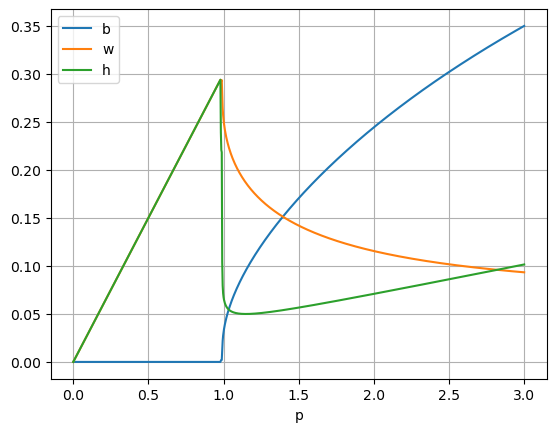
\includegraphics{plots/pasted2.png}

which is practically the same as what we had in the simplified model.

\subsection{Linear Stability Analysis}

The linear stability of the solution

\begin{align*}
\left.\frac{\partial F_{b}}{\partial b}\right|_{b=0,w=\frac{p}{\nu},h=\frac{p}{\alpha f}} & =\nu w-\nu-1=p-1\\
\left.\frac{\partial F_{b}}{\partial w}\right|_{b=0,w=\frac{p}{\nu},h=\frac{p}{\alpha f}} & =\nu\left(1+\eta b\right)^{2}b\left(1-b\right)=0\\
\left.\frac{\partial F_{b}}{\partial h}\right|_{b=0,w=\frac{p}{\nu},h=\frac{p}{\alpha f}} & =0
\end{align*}

\[
\frac{dI}{db}=-\alpha q\frac{f-1}{\left(b+q\right)^{2}}
\]

\begin{align*}
\left.\frac{\partial F_{w}}{\partial b}\right|_{b=0,w=\frac{p}{\nu},h=\frac{p}{\alpha f}} & =-\alpha q\frac{f-1}{\left(b+q\right)^{2}}h-\gamma w\left(1+\eta b\right)\left(1+3\eta b\right)\\
 & =-\alpha\frac{f-1}{q}\frac{p}{\alpha f}-\gamma\frac{p}{\nu}\\
 & =\frac{1-f}{f}\frac{p}{q}-\frac{\gamma}{\nu}p\\
 & =\left(\frac{1-f}{f}-\frac{\gamma}{\nu}\right)p\\
\left.\frac{\partial F_{w}}{\partial w}\right|_{b=0,w=\frac{p}{\nu},h=\frac{p}{\alpha f}} & =-\nu-G_{w}=-\nu\\
\left.\frac{\partial F_{w}}{\partial h}\right|_{b=0,w=\frac{p}{\nu},h=\frac{p}{\alpha f}} & =I=\alpha f
\end{align*}

\begin{align*}
\left.\frac{\partial F_{h}}{\partial b}\right|_{b=0,w=\frac{p}{\nu},h=\frac{p}{\alpha f}} & =-\alpha q\frac{f-1}{\left(b+q\right)^{2}}h\\
 & =-\alpha\frac{f-1}{q}\frac{p}{\alpha f}\\
 & =\frac{1-f}{f}\frac{1}{q}p\\
\left.\frac{\partial F_{h}}{\partial w}\right|_{b=0,w=\frac{p}{\nu},h=\frac{p}{\alpha f}} & =0\\
\left.\frac{\partial F_{h}}{\partial h}\right|_{b=0,w=\frac{p}{\nu},h=\frac{p}{\alpha f}} & =-I=-\alpha f
\end{align*}

\[
\Rightarrow J=\left[\begin{array}{ccc}
p-1 & 0 & 0\\
-\frac{\gamma}{\nu}p & -\nu & \alpha f\\
\frac{1-f}{f}\frac{1}{q}p & 0 & -\alpha f
\end{array}\right]
\]

The eigenvalues are:

\begin{align*}
\left|J-\sigma I\right| & =\left|\begin{array}{ccc}
p-1-\sigma & 0 & 0\\
-\frac{\gamma}{\nu}p & -\nu-\sigma & \alpha f\\
\frac{1-f}{f}\frac{1}{q}p & 0 & -\alpha f-\sigma
\end{array}\right|\\
 & =-\left(\nu+\sigma\right)\left|\begin{array}{cc}
p-1-\sigma & 0\\
\frac{1-f}{f}\frac{1}{q}p & -\alpha f-\sigma
\end{array}\right|\\
 & =\left(\nu+\sigma\right)\left(p-1-\sigma\right)\left(\alpha f+\sigma\right)
\end{align*}

So the eigenvalues are:

\[
\sigma=-\nu,p-1,-\alpha f
\]

Because $\nu,\alpha,f>0$, the state is stable for $p-1<0\Rightarrow p<1$.
